\chapter{Mathematical Foundations and Formulations}
\label{chap:math}

A robust real-time rendering engine is founded upon rigorous geometric algebra and optical physics. This chapter details every mathematical model implemented in \textit{Matsuri Nights}, providing step-by-step derivations alongside exact source code citations.

\section{Hierarchical Model Transformation Matrix (TRS)}
\subsection{Mathematical Formulation}
To place a 3D geometric mesh into world space, vertices undergo affine transformations comprising scale, rotation, and translation. In this engine, rotation is represented using Euler angles $(\theta_x, \theta_y, \theta_z)$ corresponding to Pitch, Yaw, and Roll in degrees. To avoid gimbal lock and maintain consistent architectural orientation, rotations are evaluated in the standard fixed-axis Euler order: \textbf{Yaw ($Y$) $\to$ Pitch ($X$) $\to$ Roll ($Z$)}.

Given local position vector $\mathbf{p} = [p_x, p_y, p_z]^T$, rotation angles $[\theta_x, \theta_y, \theta_z]^T$, and scaling vector $\mathbf{s} = [s_x, s_y, s_z]^T$, the component transformation matrices are:
\begin{equation}
\mathbf{T}(\mathbf{p}) = \begin{bmatrix}
1 & 0 & 0 & p_x \\
0 & 1 & 0 & p_y \\
0 & 0 & 1 & p_z \\
0 & 0 & 0 & 1
\end{bmatrix}, \quad
\mathbf{S}(\mathbf{s}) = \begin{bmatrix}
s_x & 0 & 0 & 0 \\
0 & s_y & 0 & 0 \\
0 & 0 & s_z & 0 \\
0 & 0 & 0 & 1
\end{bmatrix}
\end{equation}
The elementary rotation matrices about the coordinate axes are defined as:
\begin{equation}
\mathbf{R}_y(\theta_y) = \begin{bmatrix}
\cos\theta_y & 0 & \sin\theta_y & 0 \\
0 & 1 & 0 & 0 \\
-\sin\theta_y & 0 & \cos\theta_y & 0 \\
0 & 0 & 0 & 1
\end{bmatrix}, \quad
\mathbf{R}_x(\theta_x) = \begin{bmatrix}
1 & 0 & 0 & 0 \\
0 & \cos\theta_x & -\sin\theta_x & 0 \\
0 & \sin\theta_x & \cos\theta_x & 0 \\
0 & 0 & 0 & 1
\end{bmatrix}, \quad
\mathbf{R}_z(\theta_z) = \begin{bmatrix}
\cos\theta_z & -\sin\theta_z & 0 & 0 \\
\sin\theta_z & \cos\theta_z & 0 & 0 \\
0 & 0 & 1 & 0 \\
0 & 0 & 0 & 1
\end{bmatrix}
\end{equation}
The local affine model matrix $\mathbf{M}_{\text{local}}$ is composed in column-major order as:
\begin{equation}
\mathbf{M}_{\text{local}} = \mathbf{T}(\mathbf{p}) \cdot \mathbf{R}_y(\theta_y) \cdot \mathbf{R}_x(\theta_x) \cdot \mathbf{R}_z(\theta_z) \cdot \mathbf{S}(\mathbf{s})
\label{eq:trs_local}
\end{equation}
When an object is embedded as a child node within the scene graph tree, its world matrix $\mathbf{M}_{\text{world}}$ is computed recursively by pre-multiplying its parent's world matrix:
\begin{equation}
\mathbf{M}_{\text{world}} = \mathbf{M}_{\text{parent}} \cdot \mathbf{M}_{\text{local}}
\label{eq:trs_world}
\end{equation}

\subsection{Exact Code Citation}
\begin{itemize}
    \item \textbf{Local TRS Matrix Construction:} \texttt{src/Transform.h: lines 36--46} in \texttt{Transform::getLocalMatrix()}
    \item \textbf{Hierarchical World Matrix Composition:} \texttt{src/SceneNode.h: line 148} in \texttt{SceneNode::updateWorldMatrix()}
\end{itemize}

\section{Normal Transformation Matrix Derivation}
\subsection{Mathematical Formulation}
When a surface undergoes non-uniform scaling ($\mathbf{s}_x \neq \mathbf{s}_y \neq \mathbf{s}_z$), multiplying the surface normal $\mathbf{N}$ directly by the $3\times 3$ model matrix $\mathbf{M}$ breaks orthogonality with the surface tangent vector $\mathbf{T}$.

Let $\mathbf{T}$ be any tangent vector on the primitive surface satisfying $\mathbf{N}^T \mathbf{T} = 0$. Under affine transformation matrix $\mathbf{M}$, the transformed tangent vector becomes $\mathbf{T}' = \mathbf{M} \mathbf{T}$. We seek a transformation matrix $\mathbf{Q}$ for the normal such that $\mathbf{N}' = \mathbf{Q} \mathbf{N}$ maintains orthogonality:
\begin{equation}
(\mathbf{N}')^T \mathbf{T}' = 0 \implies (\mathbf{Q} \mathbf{N})^T (\mathbf{M} \mathbf{T}) = 0 \implies \mathbf{N}^T \mathbf{Q}^T \mathbf{M} \mathbf{T} = 0
\end{equation}
For this identity to hold for all arbitrary surface tangent vectors $\mathbf{T}$ where $\mathbf{N}^T \mathbf{T} = 0$, we require:
\begin{equation}
\mathbf{Q}^T \mathbf{M} = \mathbf{I} \implies \mathbf{Q}^T = \mathbf{M}^{-1} \implies \mathbf{Q} = (\mathbf{M}^{-1})^T
\label{eq:normal_matrix}
\end{equation}
Hence, surface normals must be multiplied by the \textbf{transpose of the inverse} of the upper-left $3\times 3$ model matrix:
\begin{equation}
\mathbf{N}_{\text{matrix}} = \left( (\mathbf{M}_{\text{world}}^{3\times 3})^{-1} \right)^T
\end{equation}

\subsection{Exact Code Citation}
\begin{itemize}
    \item \textbf{CPU Matrix Evaluation:} \texttt{src/SceneNode.h: line 149} in \texttt{SceneNode::updateWorldMatrix()}
    \item \textbf{GPU Normal Transformation:} \texttt{shaders/basic.vert: line 20} in \texttt{main()}:
    \begin{lstlisting}[language=GLSL, basicstyle=\ttfamily\scriptsize]
    Normal = normalMatrix * aNormal;
    \end{lstlisting}
\end{itemize}

\section{Camera System: View and Projection Matrices}
\subsection{LookAt View Matrix and Gram-Schmidt Orthonormalization}
The camera orientation is defined using Euler angles: Yaw ($\psi$, rotation around world $Y$) and Pitch ($\theta$, elevation angle), where Pitch is clamped to $[-89.0^\circ, +89.0^\circ]$. The unnormalized camera gaze direction $\mathbf{f}$ is:
\begin{equation}
\begin{aligned}
f_x &= \cos(\psi) \cdot \cos(\theta) \\
f_y &= \sin(\theta) \\
f_z &= \sin(\psi) \cdot \cos(\theta)
\end{aligned}
\end{equation}
The camera orthonormal coordinate basis $\{\mathbf{F}, \mathbf{R}, \mathbf{U}\}$ is established via the Gram-Schmidt process against the global up vector $\mathbf{U}_{\text{world}} = [0, 1, 0]^T$:
\begin{equation}
\mathbf{F} = \frac{\mathbf{f}}{\|\mathbf{f}\|}, \quad
\mathbf{R} = \frac{\mathbf{F} \times \mathbf{U}_{\text{world}}}{\|\mathbf{F} \times \mathbf{U}_{\text{world}}\|}, \quad
\mathbf{U} = \frac{\mathbf{R} \times \mathbf{F}}{\|\mathbf{R} \times \mathbf{F}\|}
\end{equation}
The view matrix $\mathbf{V}$, which transforms world coordinates into view/camera space given camera position $\mathbf{P}$, is formulated as:
\begin{equation}
\mathbf{V} = \begin{bmatrix}
R_x & R_y & R_z & -\mathbf{R}\cdot\mathbf{P} \\
U_x & U_y & U_z & -\mathbf{U}\cdot\mathbf{P} \\
-F_x & -F_y & -F_z & \mathbf{F}\cdot\mathbf{P} \\
0 & 0 & 0 & 1
\end{bmatrix}
\label{eq:view_matrix}
\end{equation}

\subsection{Perspective Projection Matrix}
The perspective projection matrix maps the viewing frustum onto Normalized Device Coordinates (NDC) $[-1, 1]^3$. With field-of-view angle $\alpha_{\text{fov}} = 45^\circ$, aspect ratio $a = \frac{\text{SCR\_WIDTH}}{\text{SCR\_HEIGHT}} = \frac{1280}{720} \approx 1.7778$, near clipping plane $z_n = 0.1\,\text{m}$, and far plane $z_f = 300.0\,\text{m}$:
\begin{equation}
\mathbf{P}_{\text{proj}} = \begin{bmatrix}
\frac{1}{a \tan(\alpha_{\text{fov}} / 2)} & 0 & 0 & 0 \\
0 & \frac{1}{\tan(\alpha_{\text{fov}} / 2)} & 0 & 0 \\
0 & 0 & -\frac{z_f + z_n}{z_f - z_n} & -\frac{2 z_f z_n}{z_f - z_n} \\
0 & 0 & -1 & 0
\end{bmatrix}
\label{eq:projection_matrix}
\end{equation}

\subsection{Exact Code Citation}
\begin{itemize}
    \item \textbf{View Matrix:} \texttt{src/Camera.h: lines 48--51} in \texttt{Camera::GetViewMatrix()}
    \item \textbf{Projection Matrix:} \texttt{src/Camera.h: lines 53--56} in \texttt{Camera::GetProjectionMatrix()}
    \item \textbf{Basis Orthonormalization:} \texttt{src/Camera.h: lines 104--113} in \texttt{Camera::updateCameraVectors()}
\end{itemize}

\section{Blinn-Phong Illumination and Halfway Vector}
\subsection{Mathematical Formulation}
Standard Phong shading computes specular highlights using the reflection vector $\mathbf{R} = 2(\mathbf{N}\cdot\mathbf{L})\mathbf{N} - \mathbf{L}$, evaluating $(\mathbf{V}\cdot\mathbf{R})^{\alpha}$. However, when the angle between $\mathbf{V}$ and $\mathbf{R}$ exceeds $90^\circ$, specular reflection cuts off abruptly. The \textbf{Blinn-Phong} model remedies this by introducing the unit \textbf{halfway vector} $\mathbf{H}$, pointing halfway between the light direction $\mathbf{L}$ and the camera view vector $\mathbf{V}$:
\begin{equation}
\mathbf{H} = \frac{\mathbf{L} + \mathbf{V}}{\|\mathbf{L} + \mathbf{V}\|}
\label{eq:halfway_vector}
\end{equation}

\begin{figure}[H]
\centering
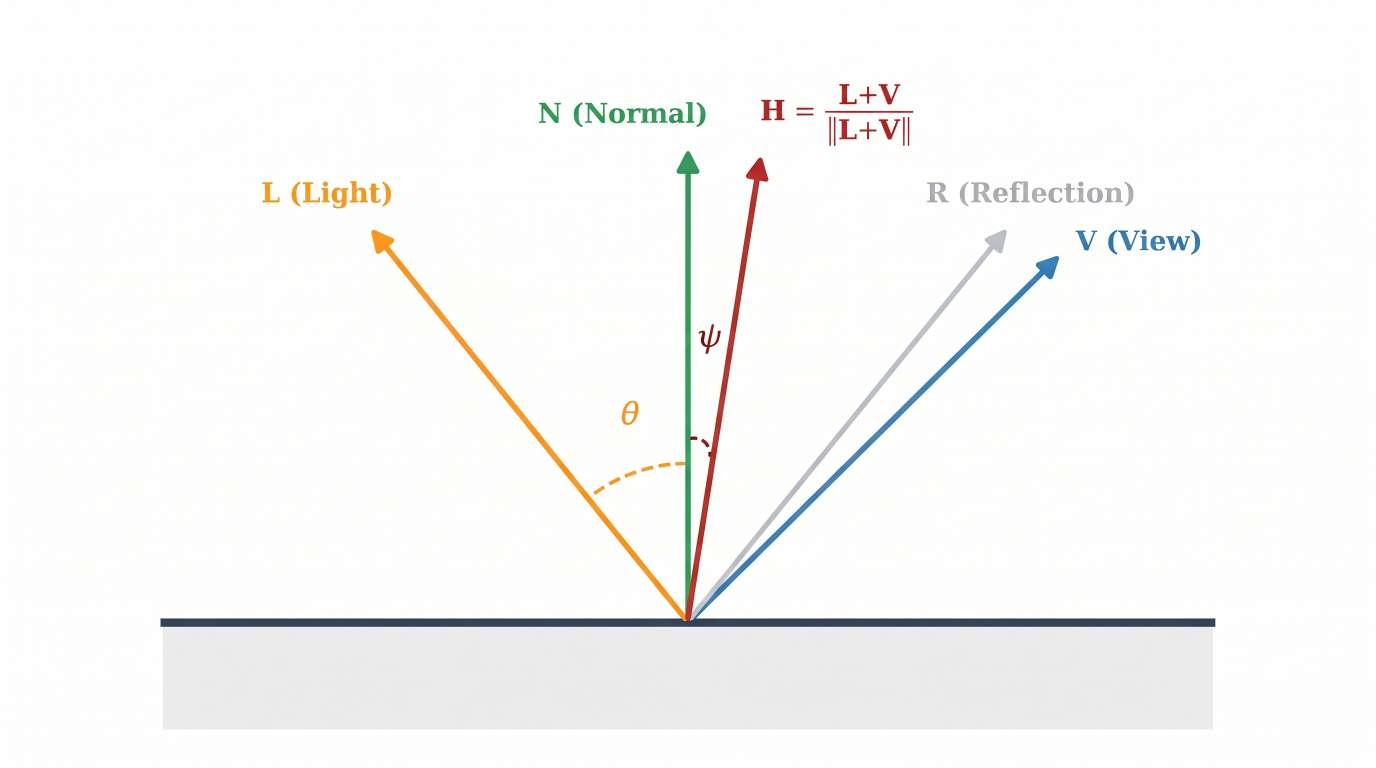
\includegraphics[width=0.55\textwidth]{figures/fig_blinn_phong_vectors.pdf}
\caption{Vector geometry of the Blinn-Phong reflection model illustrating Normal $\mathbf{N}$, Incident Light $\mathbf{L}$, View Direction $\mathbf{V}$, and the Halfway Vector $\mathbf{H}$.}
\label{fig:blinn_phong_diagram}
\end{figure}

The total illumination $I$ at a surface point is the sum of ambient, diffuse, and specular terms:
\begin{align}
I_{\text{ambient}} &= \mathbf{I}_a \otimes \mathbf{k}_d \\
I_{\text{diffuse}} &= (\mathbf{N} \cdot \mathbf{L})^+ \cdot (\mathbf{I}_d \otimes \mathbf{k}_d) \\
I_{\text{specular}} &= (\mathbf{N} \cdot \mathbf{H})^{\alpha_s} \cdot (\mathbf{I}_s \cdot k_s)
\end{align}
where $(\cdot)^+ = \max(\cdot, 0)$, $\otimes$ represents component-wise color multiplication, $\alpha_s = \text{shininess}$ (default: $32.0$), $k_s = \text{specularStrength}$ (default: $0.5$), and $\mathbf{k}_d$ is the diffuse albedo (or sampled texture color). Incorporating shadow occlusion factor $S \in [0, 1]$:
\begin{equation}
\mathbf{I}_{\text{total}} = I_{\text{ambient}} + (1 - S) \cdot \left( I_{\text{diffuse}} + I_{\text{specular}} \right)
\label{eq:blinn_phong_total}
\end{equation}

\subsection{Exact Code Citation}
\begin{itemize}
    \item \textbf{Directional Light Formulation:} \texttt{shaders/basic.frag: lines 107--131} in \texttt{CalcDirLight()}
    \item \textbf{Point Light Formulation:} \texttt{shaders/basic.frag: lines 133--165} in \texttt{CalcPointLight()}
    \item \textbf{Spotlight Formulation:} \texttt{shaders/basic.frag: lines 167--204} in \texttt{CalcSpotLight()}
\end{itemize}

\section{Point Light Attenuation and Spotlight Cone Cutoff}
\subsection{Point Light Polynomial Distance Attenuation}
As light propagates spherically through 3D space, irradiance decreases inversely with the square of the distance $d = \|\mathbf{p}_{\text{light}} - \mathbf{p}_{\text{frag}}\|$. To allow fine-grained artistic control while preventing singularities at $d \to 0$, a quadratic attenuation function is employed:
\begin{equation}
\operatorname{Att}(d) = \frac{1}{k_c + k_l d + k_q d^2}
\label{eq:attenuation}
\end{equation}
where $k_c = 1.0$ (constant term), $k_l$ is the linear factor (governing medium-range falloff), and $k_q$ is the quadratic coefficient (governing steep distance falloff). In the fragment shader, point light computations are culled early if $d^2 > 700\,\text{m}^2$ or $\operatorname{Att}(d) < 0.005$.

\subsection{Spotlight Angular Smoothstep Falloff}
The theatrical spotlight fixture emits a directed light cone along vector $\mathbf{D}_{\text{spot}}$. Let $\mathbf{L} = \frac{\mathbf{p}_{\text{light}} - \mathbf{p}_{\text{frag}}}{\|\mathbf{p}_{\text{light}} - \mathbf{p}_{\text{frag}}\|}$ be the vector from fragment to light. The angle cosine $\cos\theta = \mathbf{L} \cdot (-\mathbf{D}_{\text{spot}})$ measures deviation from the central axis.

Given an inner cutoff angle $\phi$ ($\cos\phi = \cos(15^\circ) = 0.9659$) and an outer cutoff angle $\gamma$ ($\cos\gamma = \cos(23^\circ) = 0.9205$), the smooth angular attenuation factor $I_{\text{spot}}$ is:
\begin{equation}
I_{\text{spot}} = \operatorname{clamp}\left( \frac{\cos\theta - \cos\gamma}{\cos\phi - \cos\gamma}, 0.0, 1.0 \right)
\label{eq:spotlight_cutoff}
\end{equation}

\subsection{Exact Code Citation}
\begin{itemize}
    \item \textbf{Distance Attenuation:} \texttt{shaders/basic.frag: line 143} in \texttt{CalcPointLight()}
    \item \textbf{Spotlight Cutoff Cosine:} \texttt{shaders/basic.frag: lines 178--181} in \texttt{CalcSpotLight()}
\end{itemize}

\section{16-Sample Percentage-Closer Filtering (PCF) Soft Shadows}
\subsection{Mathematical Formulation}
Standard shadow mapping projects a fragment into directional light clip space $\mathbf{p}_{\text{lightSpace}} = \mathbf{M}_{\text{lightSpace}} \cdot \mathbf{p}_{\text{world}}$. After perspective division $\mathbf{p}_{\text{proj}} = \mathbf{p}_{\text{lightSpace}}.xyz / \mathbf{p}_{\text{lightSpace}}.w$ and mapping to the $[0, 1]^3$ texture coordinate range, the fragment's light-space depth $z_{\text{proj}}$ is compared against the stored shadow map depth $D(u, v)$.

To prevent \textit{shadow acne} caused by discrete depth buffer discretization, an adaptive slope-scale normal bias is applied:
\begin{equation}
\text{bias} = \max\left( 0.0035 \cdot (1.0 - \mathbf{N}\cdot\mathbf{L}), 0.0006 \right)
\label{eq:shadow_bias}
\end{equation}
To eliminate harsh, aliased shadow silhouettes, the engine evaluates a \textbf{16-sample Percentage-Closer Filter (PCF)} across a $4\times 4$ kernel centered on the projected coordinates with disc spread radius $\Delta = \frac{1.2}{2048}$:
\begin{equation}
S(\mathbf{p}) = \frac{1}{16} \sum_{x=-1}^{2} \sum_{y=-1}^{2} \operatorname{Step}\left( z_{\text{proj}} - \text{bias} - D\left( u + x\Delta, v + y\Delta \right) \right)
\label{eq:pcf_formula}
\end{equation}
where $\operatorname{Step}(w) = 1.0$ if $w > 0$ (in shadow), and $0.0$ otherwise.

\begin{figure}[H]
\centering
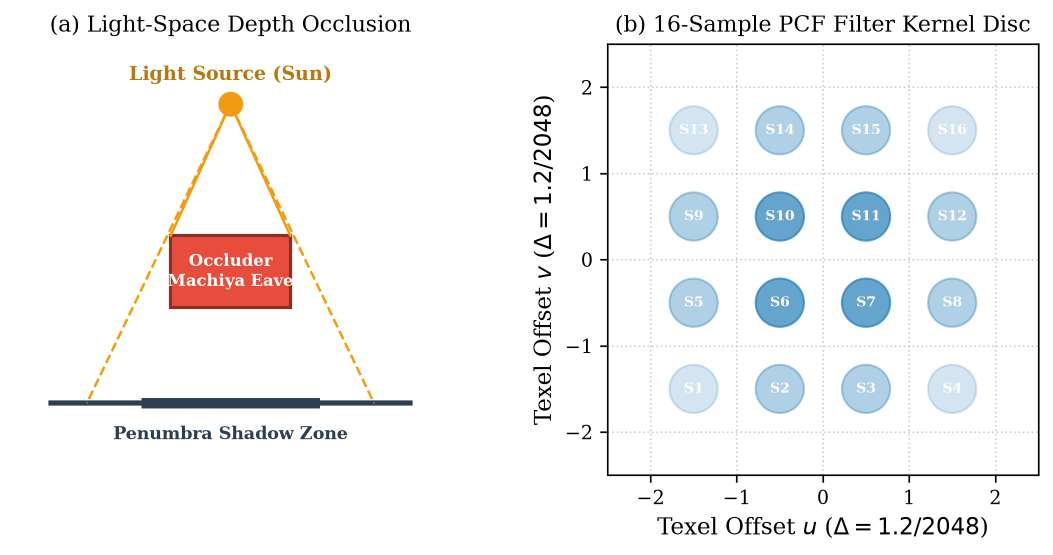
\includegraphics[width=0.88\textwidth]{figures/fig_shadow_pcf.pdf}
\caption{(a) Light-space orthographic depth occlusion geometry; (b) 16-sample PCF filter kernel sampling disk.}
\label{fig:pcf_diagram}
\end{figure}

\subsection{Exact Code Citation}
\begin{itemize}
    \item \textbf{Slope Bias \& 16-Sample PCF:} \texttt{shaders/basic.frag: lines 74--105} in \texttt{calculateShadow()}
\end{itemize}

\section{Analytical Ray-Primitive Intersections for Ray Tracing}
Both the real-time GPU ray tracer (\texttt{shaders/raytrace.frag}) and the multi-threaded CPU snapshot engine (\texttt{src/RayTracer.h}) evaluate exact analytical ray-primitive intersection formulas. Let a 3D ray be parameterized as $\mathbf{r}(t) = \mathbf{o} + t \mathbf{d}$, with $t > 0$ and $\|\mathbf{d}\| = 1$.

\subsection{Analytical Ray-Sphere Intersection}
A sphere is defined by center $\mathbf{c}$ and radius $R$: $\|\mathbf{p} - \mathbf{c}\|^2 = R^2$. Substituting the ray equation:
\begin{equation}
\|(\mathbf{o} - \mathbf{c}) + t \mathbf{d}\|^2 = R^2
\end{equation}
Let $\mathbf{v} = \mathbf{o} - \mathbf{c}$. Expanding the dot product yields the quadratic equation $t^2 + 2(\mathbf{v}\cdot\mathbf{d})t + (\|\mathbf{v}\|^2 - R^2) = 0$.
Defining coefficients $b = \mathbf{v}\cdot\mathbf{d}$ and $c = \|\mathbf{v}\|^2 - R^2$, the discriminant is:
\begin{equation}
\Delta = b^2 - c
\end{equation}
If $\Delta < 0$, the ray misses the sphere. If $\Delta \ge 0$, the nearest valid intersection distance $t$ and normal $\mathbf{N}$ are:
\begin{equation}
t = -b - \sqrt{\Delta}, \quad \mathbf{N} = \frac{\mathbf{r}(t) - \mathbf{c}}{R}
\label{eq:ray_sphere}
\end{equation}
If $t < 0.002$ (self-intersection avoidance), the secondary root $t = -b + \sqrt{\Delta}$ is tested.

\subsection{Kay-Kajiya Ray-AABB Slab Intersection}
An Axis-Aligned Bounding Box (AABB) is defined by bounds $[\mathbf{b}_{\min}, \mathbf{b}_{\max}]$. The box is treated as the intersection of three orthogonal pairs of parallel infinite slabs. For each coordinate axis $i \in \{x, y, z\}$:
\begin{equation}
t_{0, i} = \frac{b_{\min, i} - o_i}{d_i}, \quad t_{1, i} = \frac{b_{\max, i} - o_i}{d_i}
\end{equation}
Ordering intervals such that $t_{\min, i} = \min(t_{0, i}, t_{1, i})$ and $t_{\max, i} = \max(t_{0, i}, t_{1, i})$, the overall ray entry and exit distances are:
\begin{equation}
t_{\text{near}} = \max\left( t_{\min, x}, t_{\min, y}, t_{\min, z} \right), \quad
t_{\text{far}} = \min\left( t_{\max, x}, t_{\max, y}, t_{\max, z} \right)
\label{eq:slab_method}
\end{equation}
The ray intersects the AABB if and only if $t_{\text{near}} \le t_{\text{far}}$ and $t_{\text{far}} > 0.002$. The outward normal $\mathbf{N}$ is determined by identifying which slab boundary was struck at $t = t_{\text{near}}$.

\subsection{Analytical Ray-Cylinder Intersection with Height Clamping}
A vertical cylinder of radius $R$ centered at $(c_x, c_z)$ spanning $y \in [y_0, y_0 + h]$ satisfies $(p_x - c_x)^2 + (p_z - c_z)^2 = R^2$. Substituting ray components into the $XZ$ circular equation:
\begin{equation}
a = d_x^2 + d_z^2, \quad b = 2\left[(o_x - c_x)d_x + (o_z - c_z)d_z\right], \quad c = (o_x - c_x)^2 + (o_z - c_z)^2 - R^2
\end{equation}
The discriminant is $\Delta = b^2 - 4ac$. If $\Delta \ge 0$, the roots $t = \frac{-b \pm \sqrt{\Delta}}{2a}$ are evaluated. A root is accepted if and only if the vertical coordinate $y(t) = o_y + t d_y$ satisfies $y_0 \le y(t) \le y_0 + h$. The surface normal is $\mathbf{N} = \operatorname{normalize}([p_x - c_x, 0, p_z - c_z]^T)$.

\subsection{Exact Code Citation}
\begin{itemize}
    \item \textbf{GPU Ray-Sphere Intersection:} \texttt{shaders/raytrace.frag: lines 41--55}
    \item \textbf{GPU Ray-Box Slab Intersection:} \texttt{shaders/raytrace.frag: lines 58--84}
    \item \textbf{GPU Ray-Cylinder Intersection:} \texttt{shaders/raytrace.frag: lines 87--115}
    \item \textbf{CPU Ray Tracer Equivalents:} \texttt{src/RayTracer.h: lines 41--112}
\end{itemize}

\section{Parametric Curves and Sweep Mathematics}
\subsection{Catenary Sagging Formulation}
The sacred \textit{Shimenawa} straw ropes hanging from the Torii gate and the overhead street lantern spans exhibit natural gravitational catenary sag between two pole anchors at $x = -L$ and $x = +L$ with height $y_{\text{pole}}$ and central dip $s$. The ideal hyperbolic catenary $y(x) = a \cosh(x/a) - a$ is accurately approximated using a computationally efficient second-degree parabola:
\begin{equation}
\tilde{x} = \frac{x}{L} \in [-1, 1], \quad y(x) = y_{\text{pole}} - s \cdot \left( 1 - \tilde{x}^2 \right)
\label{eq:catenary_code}
\end{equation}
The tangent vector along the curve used to orient sweeping frames is obtained by differentiation:
\begin{equation}
\frac{dy}{dx} = \frac{2 s \tilde{x}}{L} \implies \mathbf{T}(x) = \operatorname{normalize}\left( \begin{bmatrix} 1 \\ \frac{2 s \tilde{x}}{L} \\ 0 \end{bmatrix} \right)
\label{eq:catenary_tan}
\end{equation}

\begin{figure}[H]
\centering
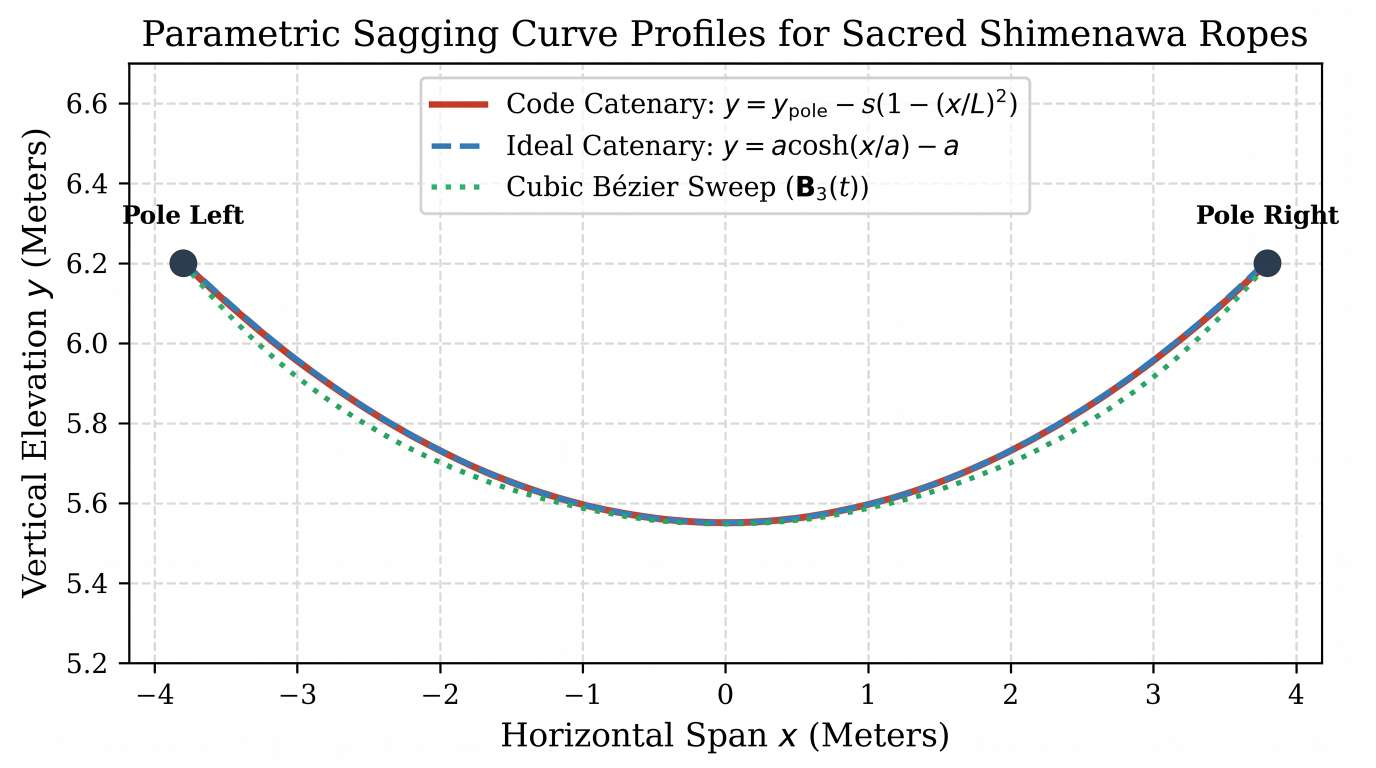
\includegraphics[width=0.62\textwidth]{figures/fig_catenary_bezier.pdf}
\caption{Comparison of the parabolic sagging curve against ideal hyperbolic catenary and cubic B\'ezier formulations.}
\label{fig:catenary_comparison}
\end{figure}

\subsection{Parametric Bézier Curves}
Quadratic and Cubic B\'ezier curves are evaluated using Bernstein polynomials:
\begin{align}
\mathbf{B}_2(t) &= (1-t)^2 \mathbf{P}_0 + 2(1-t)t \mathbf{P}_1 + t^2 \mathbf{P}_2, \quad t \in [0, 1] \\
\mathbf{B}_3(t) &= (1-t)^3 \mathbf{P}_0 + 3(1-t)^2 t \mathbf{P}_1 + 3(1-t)t^2 \mathbf{P}_2 + t^3 \mathbf{P}_3, \quad t \in [0, 1]
\label{eq:bezier_formulas}
\end{align}
Their first derivatives yield the local curve tangent vector $\mathbf{T}(t) = \operatorname{normalize}(\mathbf{B}'(t))$.

\subsection{Bishop Frame Parallel Transport}
Standard Frenet-Serret reference frames $(\mathbf{T}, \mathbf{N}, \mathbf{B})$ fail when a 3D spline curve undergoes inflection points ($\kappa = 0$), causing the normal vector to flip $180^\circ$ and producing catastrophic pinching or twisting in swept tubes. To guarantee rotation-minimizing swept meshes, \textit{Matsuri Nights} implements \textbf{Bishop frame parallel transport}:

Given an arbitrary initial normal $\mathbf{N}_0 \perp \mathbf{T}_0$, subsequent normals $\mathbf{N}_{i+1}$ along discretized curve points $\mathbf{P}_i$ are transported via the minimum-rotation axis $\mathbf{A} = \mathbf{T}_i \times \mathbf{T}_{i+1}$:
\begin{equation}
\theta_i = \arccos\left( \mathbf{T}_i \cdot \mathbf{T}_{i+1} \right), \quad
\mathbf{N}_{i+1} = \operatorname{Rotate}\left( \mathbf{N}_i, \theta_i, \operatorname{normalize}(\mathbf{A}) \right), \quad
\mathbf{B}_{i+1} = \mathbf{T}_{i+1} \times \mathbf{N}_{i+1}
\label{eq:bishop_frame}
\end{equation}

\subsection{Parabolic Projectile Kinematics for Hopping Takoyaki Balls}
Each of the 6 food balls on the Takoyaki stall griddle executes continuous jumping motion. The vertical hop elevation $\Delta y(t)$ is parameterized across period $T = 0.95\,\text{s}$ with apex height $h_{\text{max}} = 0.18\,\text{m}$ as:
\begin{equation}
\tau = \frac{t \pmod T}{T} \in [0, 1], \quad \Delta y(\tau) = 4 h_{\text{max}} \cdot \tau \cdot (1 - \tau)
\label{eq:takoyaki_projectile}
\end{equation}

\subsection{Exact Code Citation}
\begin{itemize}
    \item \textbf{Catenary Sagging Curve:} \texttt{src/Curves.h: lines 613--625} in \texttt{Curves::createCatenaryRope()}
    \item \textbf{Bézier 2 \& 3 Evaluation:} \texttt{src/Curves.h: lines 37--81} in \texttt{Bezier2} and \texttt{Bezier3}
    \item \textbf{Bishop Frame Parallel Transport:} \texttt{src/Curves.h: lines 162--215} in \texttt{Curves::computeBishopFrames()}
    \item \textbf{Takoyaki Projectile Motion:} \texttt{src/Objects.h: lines 3125--3150} in \texttt{TakoyakiStall::update()}
\end{itemize}
